\documentclass{fkssolpub}

\usepackage[czech]{babel}
\usepackage{fontspec}
\usepackage{fkssugar}
\usepackage{amsmath}
\usepackage{graphicx}

\newcommand{\dd}{\mathrm{d}}
\renewcommand{\angle}{\sphericalangle}

\author{Ondřej Sedláček}
\school{Gymnázium Oty Pavla} 
\series{4}
\problem{1} 

\begin{document}

\begin{figure}
  \begin{center}
    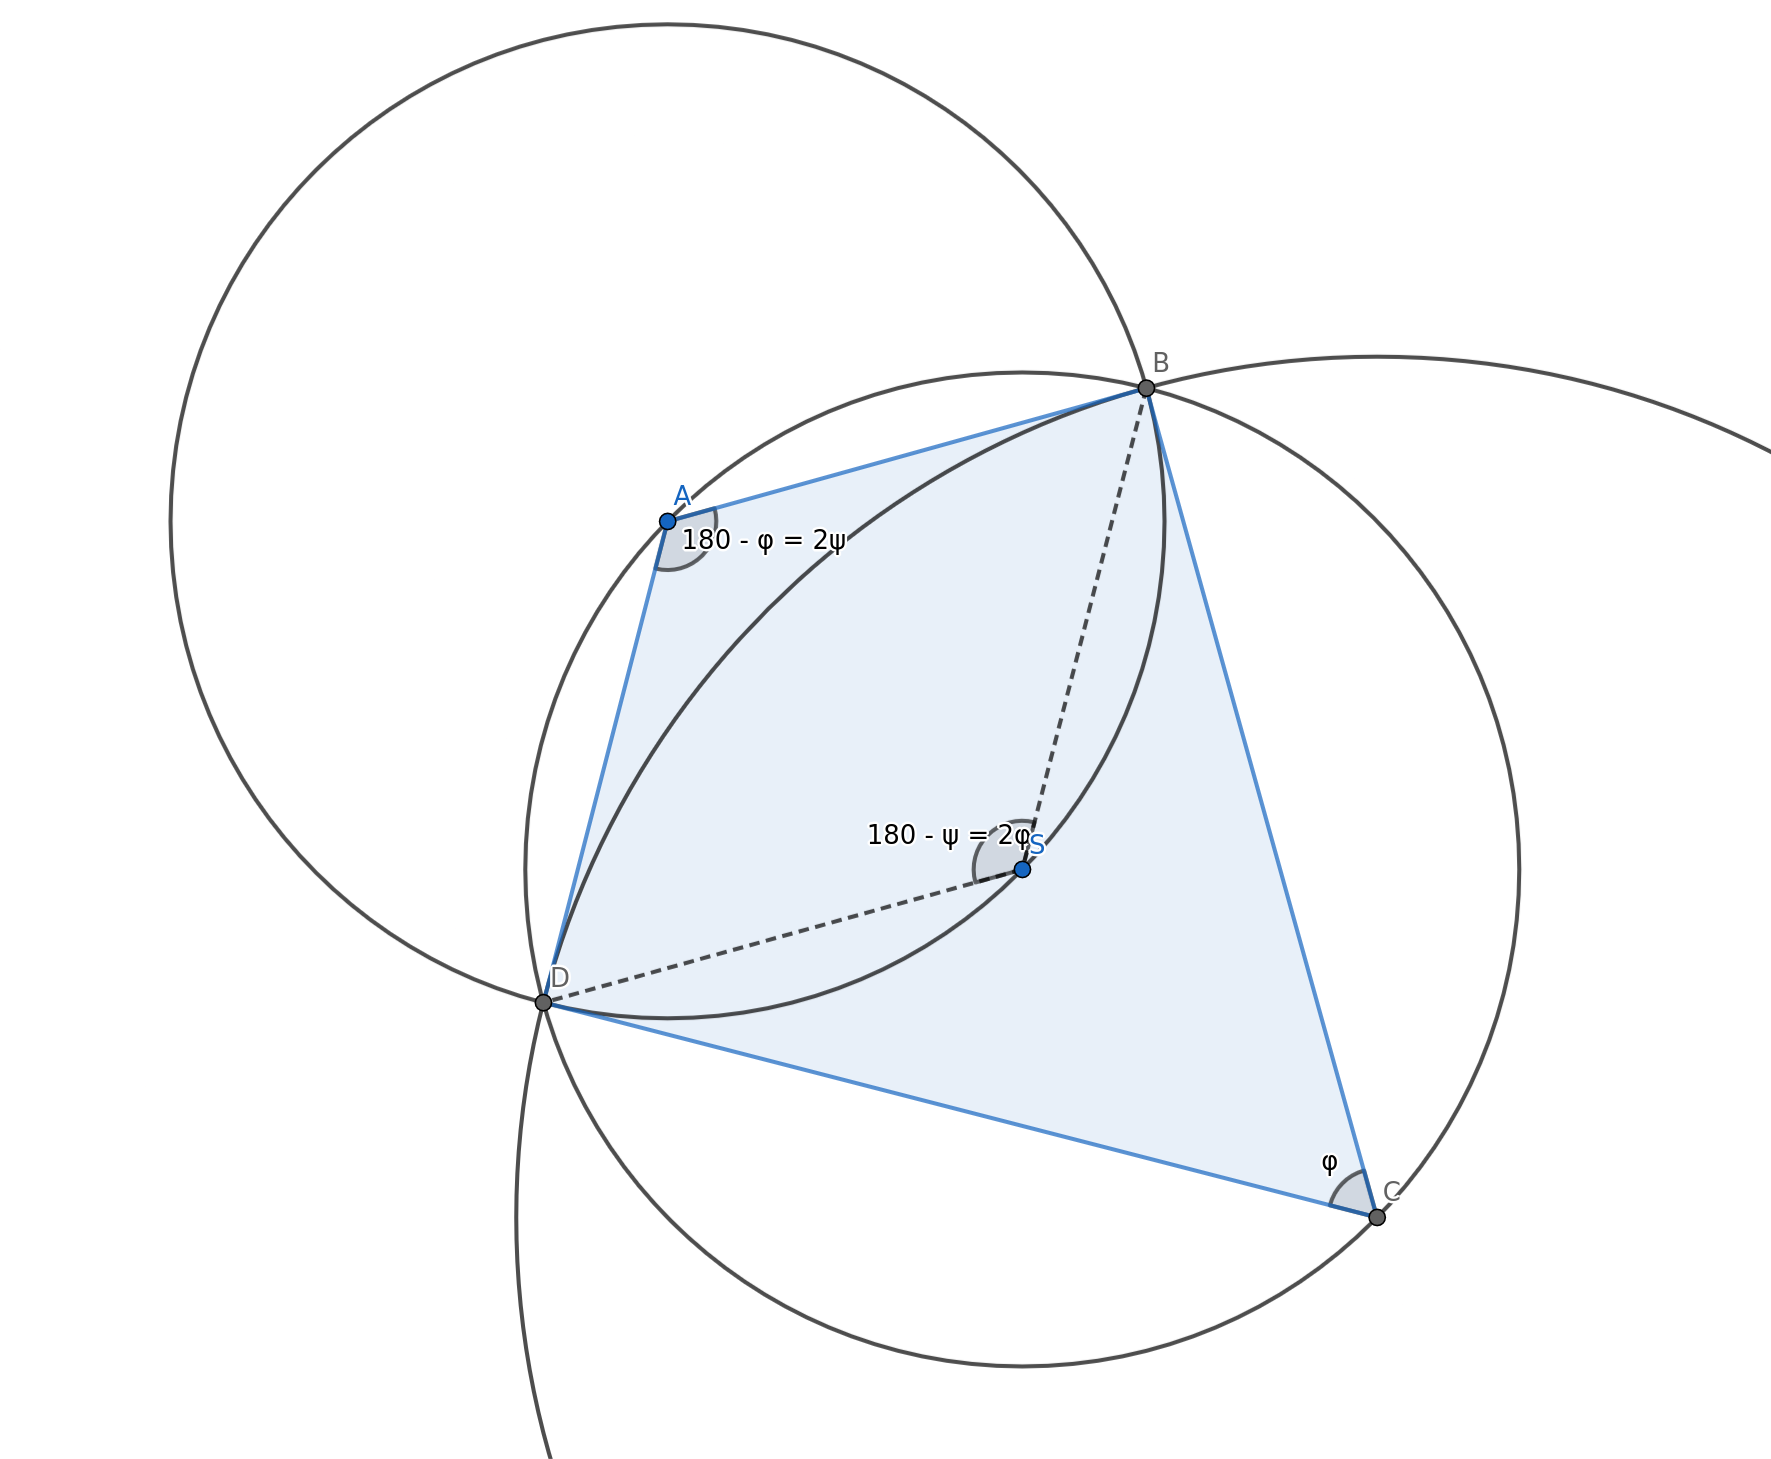
\includegraphics[width=0.95\textwidth]{1-fig.png}
  \end{center}
  \caption{Konstrukce jednoho z krajních případů}\label{fig:}
\end{figure}


Pro vyřešení nám stačí najít dva krajní případy, kdy bod $S$ buď leží na kružnici $Slovensko$, nebo na kružnici $Svet$. V intervalu mezi těmito případy pak musí nutně bod $S$ ležet v průniku těchto kruhů, protože když se bude zmenšovat středový úhel u bodu $A$, bude se poloměr kružnice $Slovensko$ zvětšovat a stejně tak u druhé kružnice.

Nechť $\phi = \frac{|\angle BAD|}{2}$ a $\psi = \frac{|\angle DSB|}{2}$. Pak v prvním krajním případě bude bod $S$ ležet na kružnici $Slovensko$, tedy z obvodových a středových úhlů platí:

\[
  2 \phi = 180^{\circ} - \psi
\]
\[
  2 \psi = 180^{\circ} - \phi
\]

Z toho dostaneme:

\[
  2 (180^{\circ} - 2 \psi) = 180^{\circ} - \psi
\]
\[
  360^{\circ} - 4 \psi = 180^{\circ} - \psi
\]
\[
  \psi = 60^{\circ} \qquad \phi = \frac{180^{\circ} - \psi}{2} = 60^{\circ}
\]

A tedy v tomto krajním případě je $|\angle BAD| = 120^{\circ}$.

Protože druhý případ je analogický s prvním krajním případem, jenom $|\angle BDC| = 120^{\circ}$, můžeme snadno dopočítat, že v tomto případě $|\angle BAD| = 60^{\circ}$.

Tedy aby bod $S$ ležel v průniku kruhů, musí platit, že $|\angle BAD| \in \langle 60^{\circ}, 120^{\circ} \rangle$.

Co se týče průniku kružnic, nemůže v něm nikdy bod $S$ ležet, protože kružnice mají nejvýše dva průniky, což kružnice $Slovensko$ a $Svet$ mají po celou dobu, pokud deltoid nezdegeneruje, a to body $B$ a $D$.

Tím je důkaz u konce.

\end{document}
